% Material found at https://www.elsevier.com/authors/author-schemas/latex-instructions

\documentclass{elsarticle}

\usepackage{lineno,hyperref}
\modulolinenumbers[5]

%=== Added for MU paper ====
\usepackage{color,soul} %% this was needed to have highlighted text
\usepackage{graphicx}
\usepackage{array,colortbl,xcolor}
\usepackage{hyperref}
\usepackage{amsmath}
\usepackage{amssymb}
\usepackage{mathtools}
\usepackage{nomencl}
\usepackage{bm}
\usepackage{subcaption}
\usepackage{systeme}
\makenomenclature
\graphicspath{{./figures/}}

\journal{Annals of Nuclear Energy}

%%%%%%%%%%%%%%%%%%%%%%%
%% Elsevier bibliography styles
%%%%%%%%%%%%%%%%%%%%%%%
%% To change the style, put a % in front of the second line of the current style and
%% remove the % from the second line of the style you would like to use.
%%%%%%%%%%%%%%%%%%%%%%%

%% Numbered
\bibliographystyle{model1-num-names}

%% Numbered without titles
%\bibliographystyle{model1a-num-names}

%% Harvard
%\bibliographystyle{model2-names.bst}\biboptions{authoryear}

%% Vancouver numbered
%\usepackage{numcompress}\bibliographystyle{model3-num-names}

%% Vancouver name/year
%\usepackage{numcompress}\bibliographystyle{model4-names}\biboptions{authoryear}

%% APA style
%\bibliographystyle{model5-names}\biboptions{authoryear}

%% AMA style
%\usepackage{numcompress}\bibliographystyle{model6-num-names}

%% `Elsevier LaTeX' style
%\bibliographystyle{elsarticle-num}
%%%%%%%%%%%%%%%%%%%%%%%

\begin{document}

\begin{frontmatter}

\title{Mining Data in a Simulation-Based PRA Framework}
%% \tnotetext[mytitlenote]{Fully documented templates are available in the elsarticle package on \href{http://www.ctan.org/tex-archive/macros/latex/contrib/elsarticle}{CTAN}.}

%% Group authors per affiliation:
\author{D. Mandelli, D. Maljovec, A. Alfonsi, C. Parisi, P. Talbot, J. Cogliati, C. Smith, C. Rabiti}
\address{Idaho National Laboratory (INL), 2525 Fremont Ave, 83402 Idaho Falls (ID), USA}

\begin{abstract}
  Risk importance measures are indexes that are used to rank systems, 
structures and components (SSCs) using risk-informed methods. 
The most used/known measures are: Risk Reduction Worth (RRW), 
Risk Achievement Worth (RAW), Birnbaum (B) and Fussell-Vesely (FV). 
Once obtained from classical Probabilistic Risk Analysis (PRA) analyses, 
these risk measures can be effectively employed to relatively rank
component importance.
In contrast to classical PRA methods, 
Dynamic PRA methods couple stochastic models with safety analysis 
codes to determine risk associate to complex systems such as nuclear 
plants. Compared to classical PRA methods, simulation-based approaches
can evaluate with 
higher resolution the safety impact of timing and sequencing of events 
on the accident progression. 
The objective of this paper is to present a series of methods that 
can be employed to measure risk importance of components which are 
part of complex systems such as nuclear power plants.
The first set of measures are directly derived from classical risk 
importance measures (e.g., RRW, RAW, B and FV) and that can be employed
to any Dynamic PRA analysis.
In addition, we provide a set of risk importance measures that capture the 
dynamic nature of the problem and provide insight related to plant safety 
margins.

\end{abstract}

\begin{keyword}
%% keywords here, in the form: keyword \sep keyword
Data Mining \sep Dynamic PRA \sep Probabilistic Risk Assessment \sep Clustering 
\end{keyword}

\end{frontmatter}

\linenumbers

\printnomenclature[1in]

\section{Introduction}
\label{sec:introduction}
RAVEN (\textbf{R}isk \textbf{A}nalysis \textbf{V}irtual \textbf{EN}vironment)~\cite{Nureg1150}  is one of the many INL-developed software tools researchers can 
use to identify and 
increase the safety margin in complex systems (e.g. Nuclear Power Plants). It is a modular or ``plug-able'' framework that can be coupled with other computer 
modeling systems. RAVEN is capable to agnostically communicate with any system 
code. This agnosticism includes providing Application Programming Interfaces (APIs). These APIs are used to allow RAVEN to interact with any code as long as all 
the parameters that need to be perturbed are accessible through input files or via python interfaces. 
As a generic software framework, RAVEN is designed to perform parametric and probabilistic analysis based on the response of complex system codes. RAVEN is 
capable of investigating the system response as well as the input space using standard sampling techniques (e.g Monte Carlo, Grid, or Latin Hyper Cube), but its 
strength is focused toward system feature discovery, such as limit surfaces (i.e. separating regions of the input space leading to system failure, using dynamic 
supervised learning techniques), and advanced data analysis methodologies (i.e. Topology-based domain decomposition, Data Mining, Clustering, etc.).

The development of RAVEN has begun in 2012 to satisfy the need to provide a modern risk evaluation framework. RAVEN principal assignment is to provide the 
necessary software and algorithms in order to employ the concept developed by the Risk Informed Safety Margin Characterization (RISMC) path-
way~\cite{RISMC}. 
RISMC is one of the pathways defined within the Light Water Reactor Sustainability (LWRS) program. In the RISMC approach, the goal is not just specifically 
identifying the frequency of an event potentially leading to a system failure, but also to analyze the ``distance'' and the drivers toward the happening of key 
safety-related events. This approach may be used in identifying and increasing the safety margins related to those events. A safety margin is a numerical value 
quantifying the probability that a safety metric (e.g. as peak pressure in a pipe) is exceeded under certain conditions. The initial development of RAVEN has 
been focused on providing dynamic risk assessment capability to RELAP-7~\cite{RELAP7}, currently under development at the INL. All the methodologies
developed have been modularized in order to be applied to any computer modeling system (e.g., BISON, RELAP-7, RELAP5-3D, MELCOR, etc.).

The aim of this manuscript is to present a peculiar capability within the RAVEN framework named \textit{``EnsembleModels''}.

RAVEN is currently able to construct multi-targets Reduced Order Models (Ref.4), which are aimed to represent the response of a system (in a 
fixed configuration) for multiple Figures of Merits (FOMs) and time-dependent ROMs (see Ref.5). These capabilities represent the initial steps for a larger 
implementation about the interaction of multiple models. In fact, in several cases, multiple models need to interface with each other since the initial conditions of 
one are dependent on the outcomes of another.
To better understand the problem that here is solved, it is useful to consider two simple examples:
\begin{enumerate}
  \item The following problem is considered: a weather forecast simulation code ``a'' is used to compute the external (i.e. ambient) temperature in a certain location. 
  A second model ``b'' is inquired to compute the average temperature in a room having as boundary condition, among several others, the external ambient 
  temperature. The response of the model ``b'' depends on the outcome of the model ``a'';
   \item Two different simulation codes are considered: a) a code that is meant to compute the thermal conductivity of the ceramic Uranium Dioxide (UO2) as 
   function of the Temperature, and b) a Thermal-hydraulic (TH) code that is used to compute the Temperature field of a reactor, whose heat conduction depends on 
   the thermal conductivity value. As easily inferable, the two models are mutual dependent, determining in a non-linear system of equations.
\end{enumerate}
The two reported examples are only aimed to illustrate the reason why the creation of a framework to make interact different models is a key development for the 
advancement of RAVEN as a comprehensive calculation flow driver. Before reporting how the ensemble-models have been implemented, it is necessary to briefly 
describe the representative Model ``entities'' that are available in RAVEN.



\begin{figure}
    \centering
    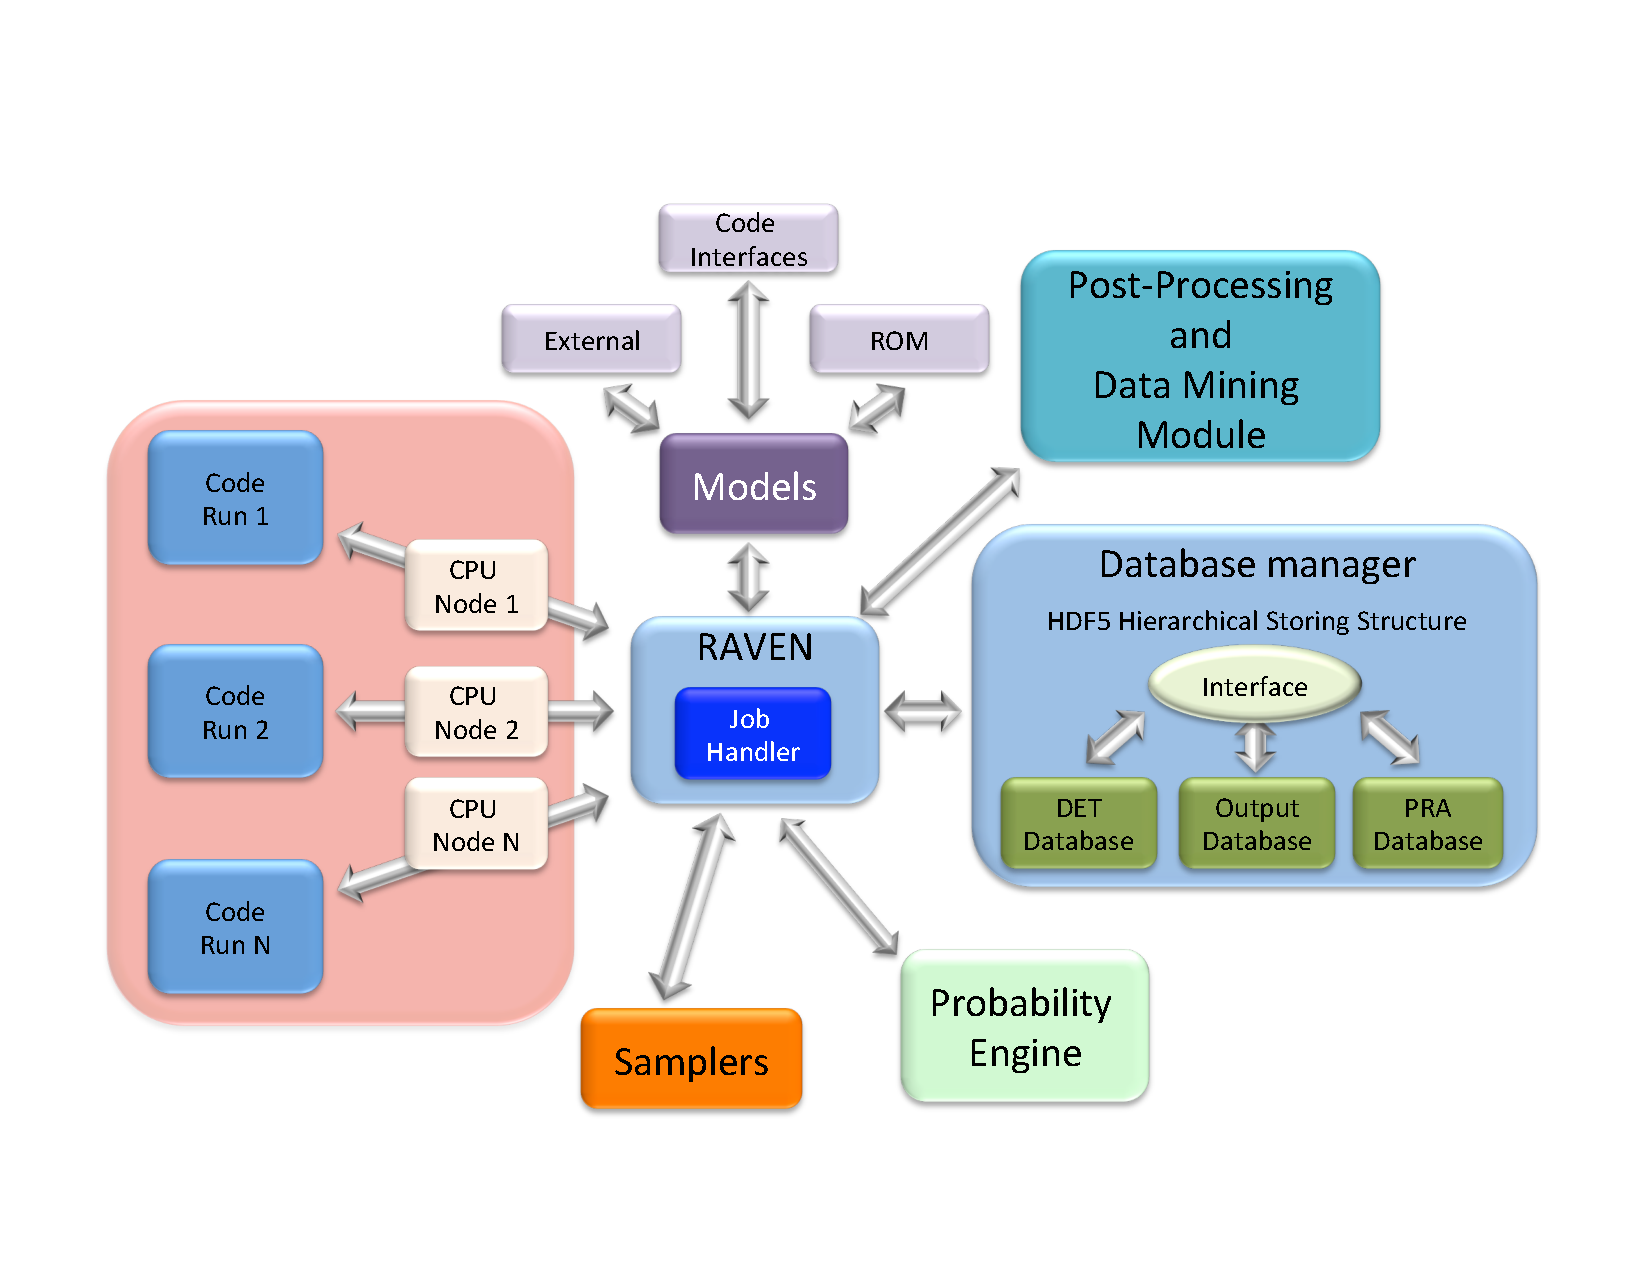
\includegraphics[scale=0.5]{raven.pdf}
    \caption{RAVEN}
    \label{fig:raven}
\end{figure}

\section{RISMC Approach to PRA}
\label{sec:rismc}

The RISMC approach~\cite{RISMC} employs both deterministic and stochastic methods 
in a single analysis framework (see Figure~\ref{fig:RISMCoverview}). In the deterministic method 
set we include:
\begin{itemize}
  \item Modeling of the thermal-hydraulic behavior of the plant~\cite{BWR_SBO_Mandelli,BWRanalysis}
  \item Modeling of external events such as flooding~\cite{mandelliPSA2015}
  \item Modeling of the operators’ responses to the accident scenario~\cite{HRA_BoringReport2014}
\end{itemize}

\begin{figure}
    \centering
    \centerline{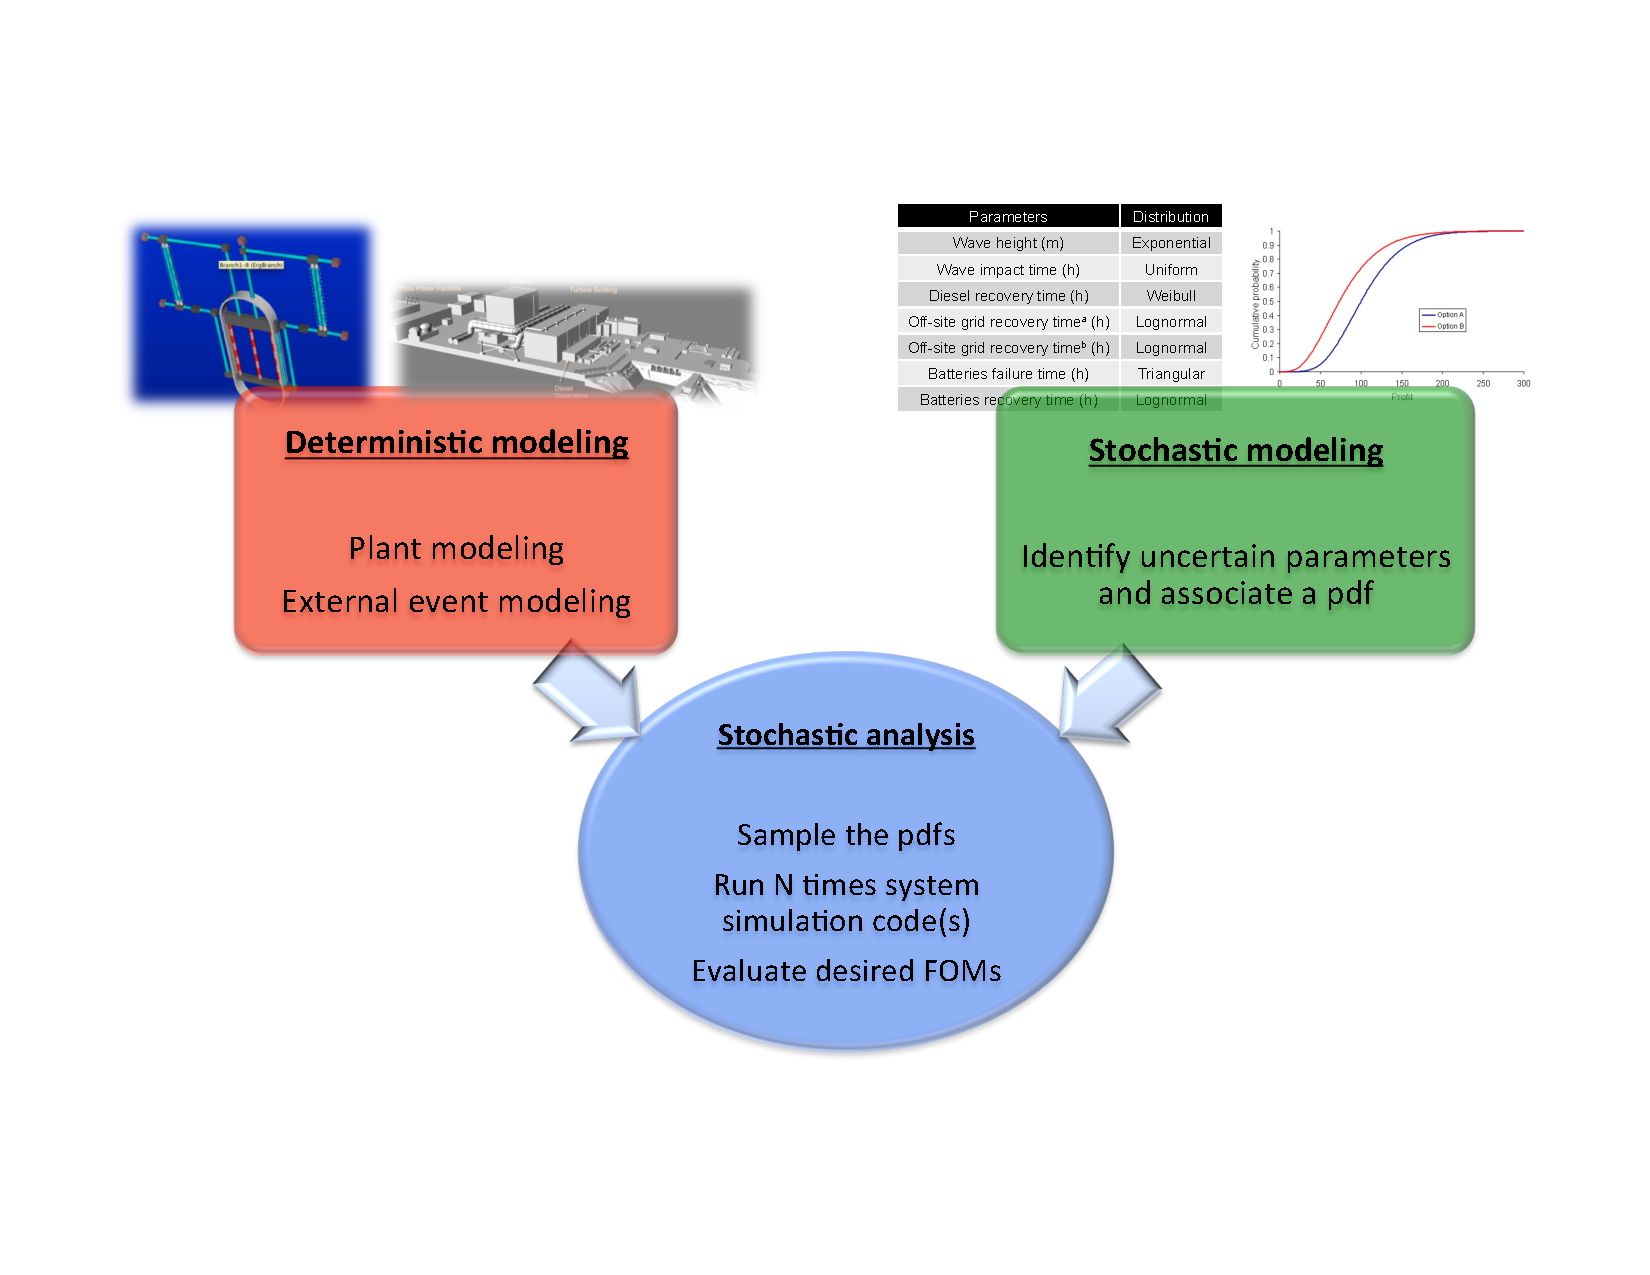
\includegraphics[scale=0.4]{RISMCoverview.pdf}}
    \caption{Overview of the RISMC approach}
    \label{fig:RISMCoverview}
\end{figure}

Note that deterministic modeling of the plant or external events can be performed by employing specific 
simulator codes but also surrogate models~\cite{ROM}, known as reduced order models (ROM). ROMs would 
be employed 
in order to decrease the high computational costs of employed codes. In addition, multi-fidelity codes 
can be employed to model the same system; the idea is to switch from low-fidelity to high-fidelity code 
when higher accuracy is needed (e.g., use low-fidelity codes for steady-state conditions and high-fidelity 
code for transient conditions)

In the stochastic modeling we include all stochastic parameters that are of interest in the PRA analysis 
such as uncertain parameters and stochastic failure of system/components.
As mentioned earlier, the RISMC approach heavily relies on multi-physics system simulator codes 
(e.g., RELAP5-3D~\cite{relap5}) coupled with stochastic analysis tools (e.g., RAVEN~\cite{raven}).  
From a PRA point of view, this type of simulation can be described by using two sets of variables:
\begin{itemize}
  \item $\boldsymbol c = \boldsymbol c(t)$ represents the status of components and systems of the simulator 
        (e.g., status of emergency core cooling system, AC system)
  \item $\boldsymbol \theta = \boldsymbol \theta (t)$ represents the temporal evolution of a simulated 
        accident scenario, i.e., $\boldsymbol \theta (t)$ represents a single simulation run. 
        Each element of $\boldsymbol \theta$ can be for example the values of temperature or pressure in 
        a specific node of the simulator nodalization.
\end{itemize}

From a mathematical point of view, a single simulator run can be represented as a single trajectory in the 
phase space. The evolution of such a trajectory in the phase space can be described as follows:
\begin{equation}
  \begin{cases}
    \dfrac{\partial \boldsymbol \theta }{\partial t}  = \boldsymbol \Xi (\boldsymbol \theta , \boldsymbol c, \boldsymbol s , t)   \\ \\ 
    \dfrac{\partial \boldsymbol c }{\partial t}  = \boldsymbol \Gamma (\boldsymbol \theta , \boldsymbol c, \boldsymbol s , t) 
  \end{cases}    
  \label{eq:trajectory}
\end{equation}
where:
\begin{itemize}
  \item $\boldsymbol \Xi$ is the actual simulator code that describes how θ evolves in time
  \item $\boldsymbol \Gamma$ is the operator which describes how c evolves in time , i.e., the status 
        of components and systems at each time step
  \item $\boldsymbol C$ is the set of stochastic parameters.
\end{itemize}

Starting from the system located in an initial state, $\boldsymbol \theta (t=0) = \boldsymbol \theta(0)$, 
and the set of stochastic parameters (which are generally generated through a stochastic sampling process), 
the simulator determine at each 
time step the temporal evolution of $\boldsymbol \theta (t)$. At the same time, the system control logic  
determines the status of the system and components $\boldsymbol c(t)$.
 
By using the RISMC approach, the PRA analysis is performed by~\cite{}:
\begin{enumerate}
  \item Associating a probabilistic distribution function (pdf) to the set of parameters 
        $\boldsymbol s$ (e.g., timing of events)
  \item Performing stochastic sampling of the pdfs defined in Step 1
  \item Performing a simulation run given $\boldsymbol s$ sampled in Step 2, i.e., solve the 
        system of equations~\ref{??}
  \item Repeating Steps 2 and 3 $M$ times and evaluating user defined stochastic parameters such 
        as core damage (CD) probability ($P_{CD}$).
\end{enumerate}

\section{RISMC Approach and Classical PRA}
\label{sec:analogy}

In order to better understand the results obtained in Section~\ref{sec:test} it is worth to illustrate 
a link between classical PRA and RISMC approach.
Let's consider a system that is composed by two components (i.e, A and B) in a series configuration where
each component has a failure probability (i.e., $p_A$ and $p_B$ respectively) as shown in Fig.~ref{}.

In a classical PRA framework such system can be modeled using a FT method that is composed by two basic events:
A failed and B failed.
System failure would be represented by a single ``AND'' gate that combine the two basic events as shown in 
Fig.~ref{}.

\begin{figure}
  \centering
  \begin{subfigure}{.5\textwidth}
    \centering
    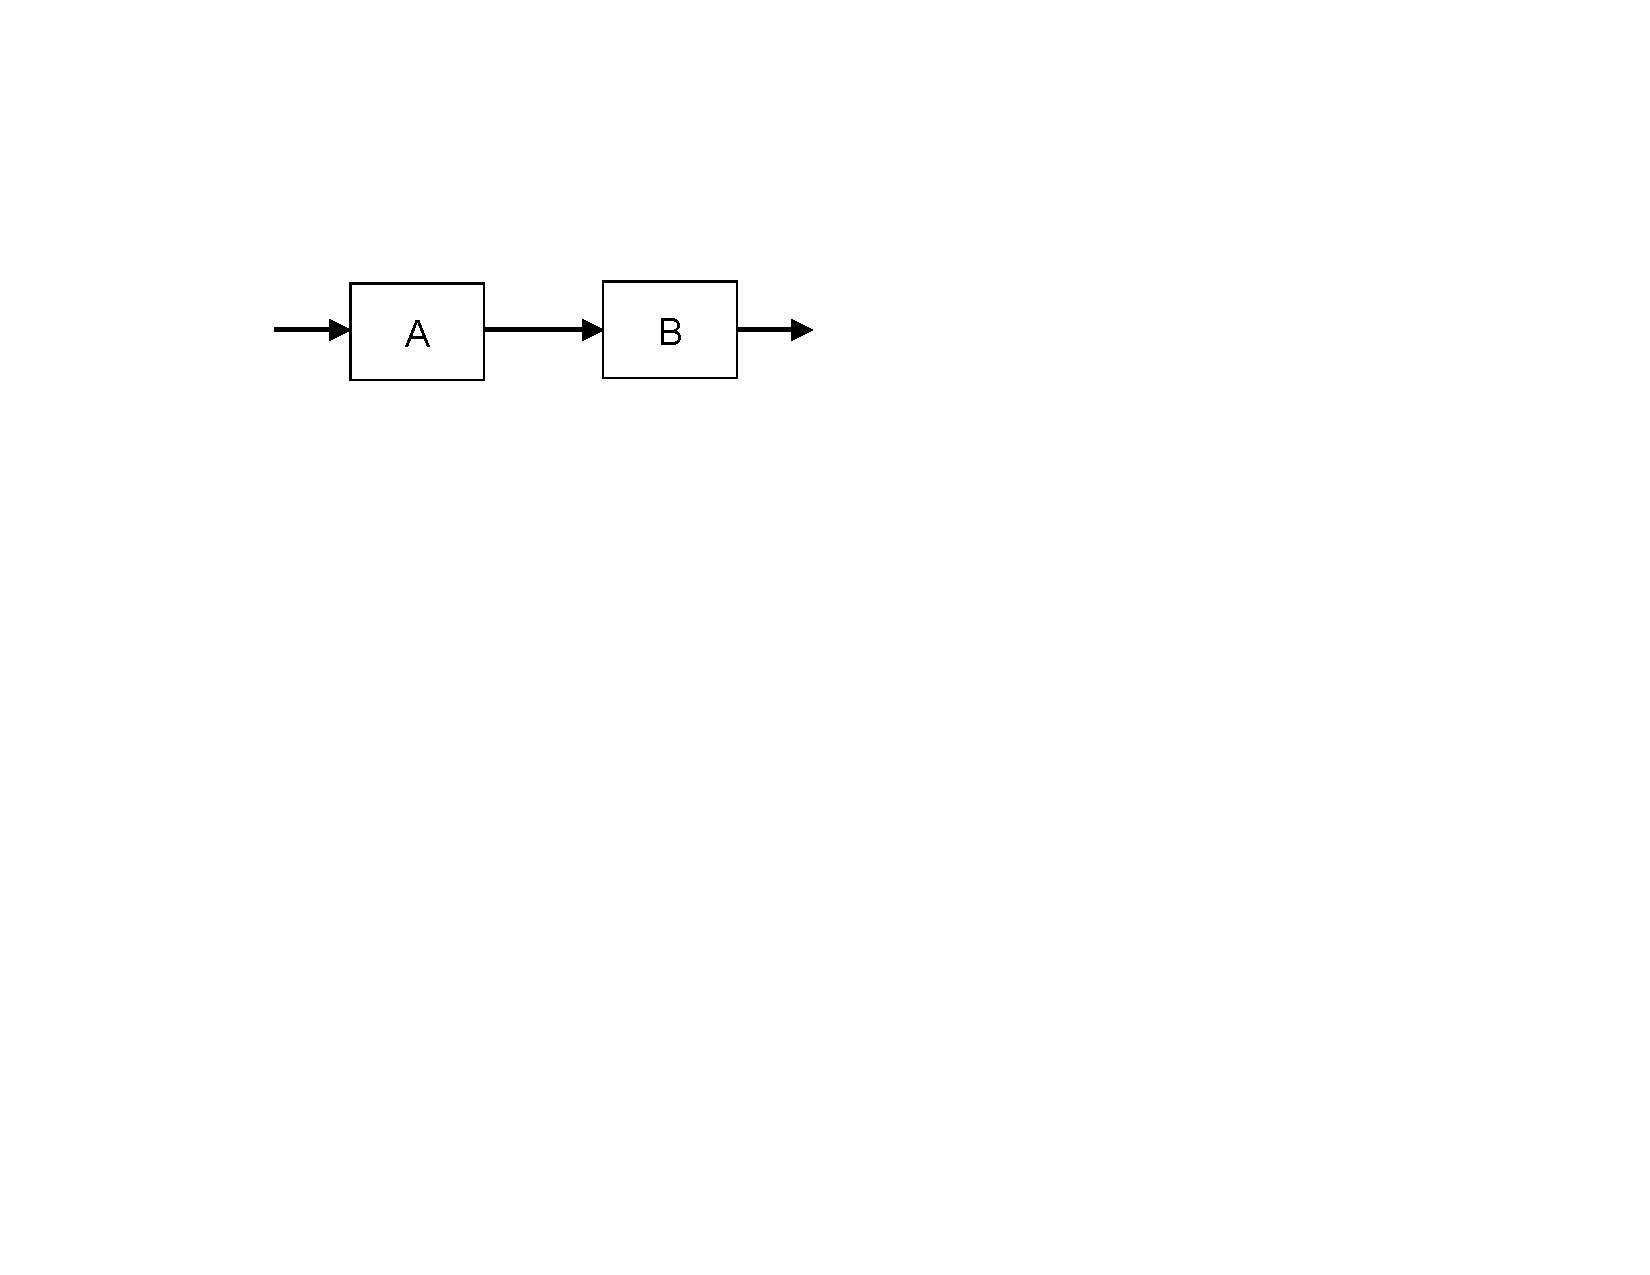
\includegraphics[scale=0.6]{ABsystem.pdf}
    \label{fig:sub1}
  \end{subfigure}%
  \begin{subfigure}{.5\textwidth}
    \centering
    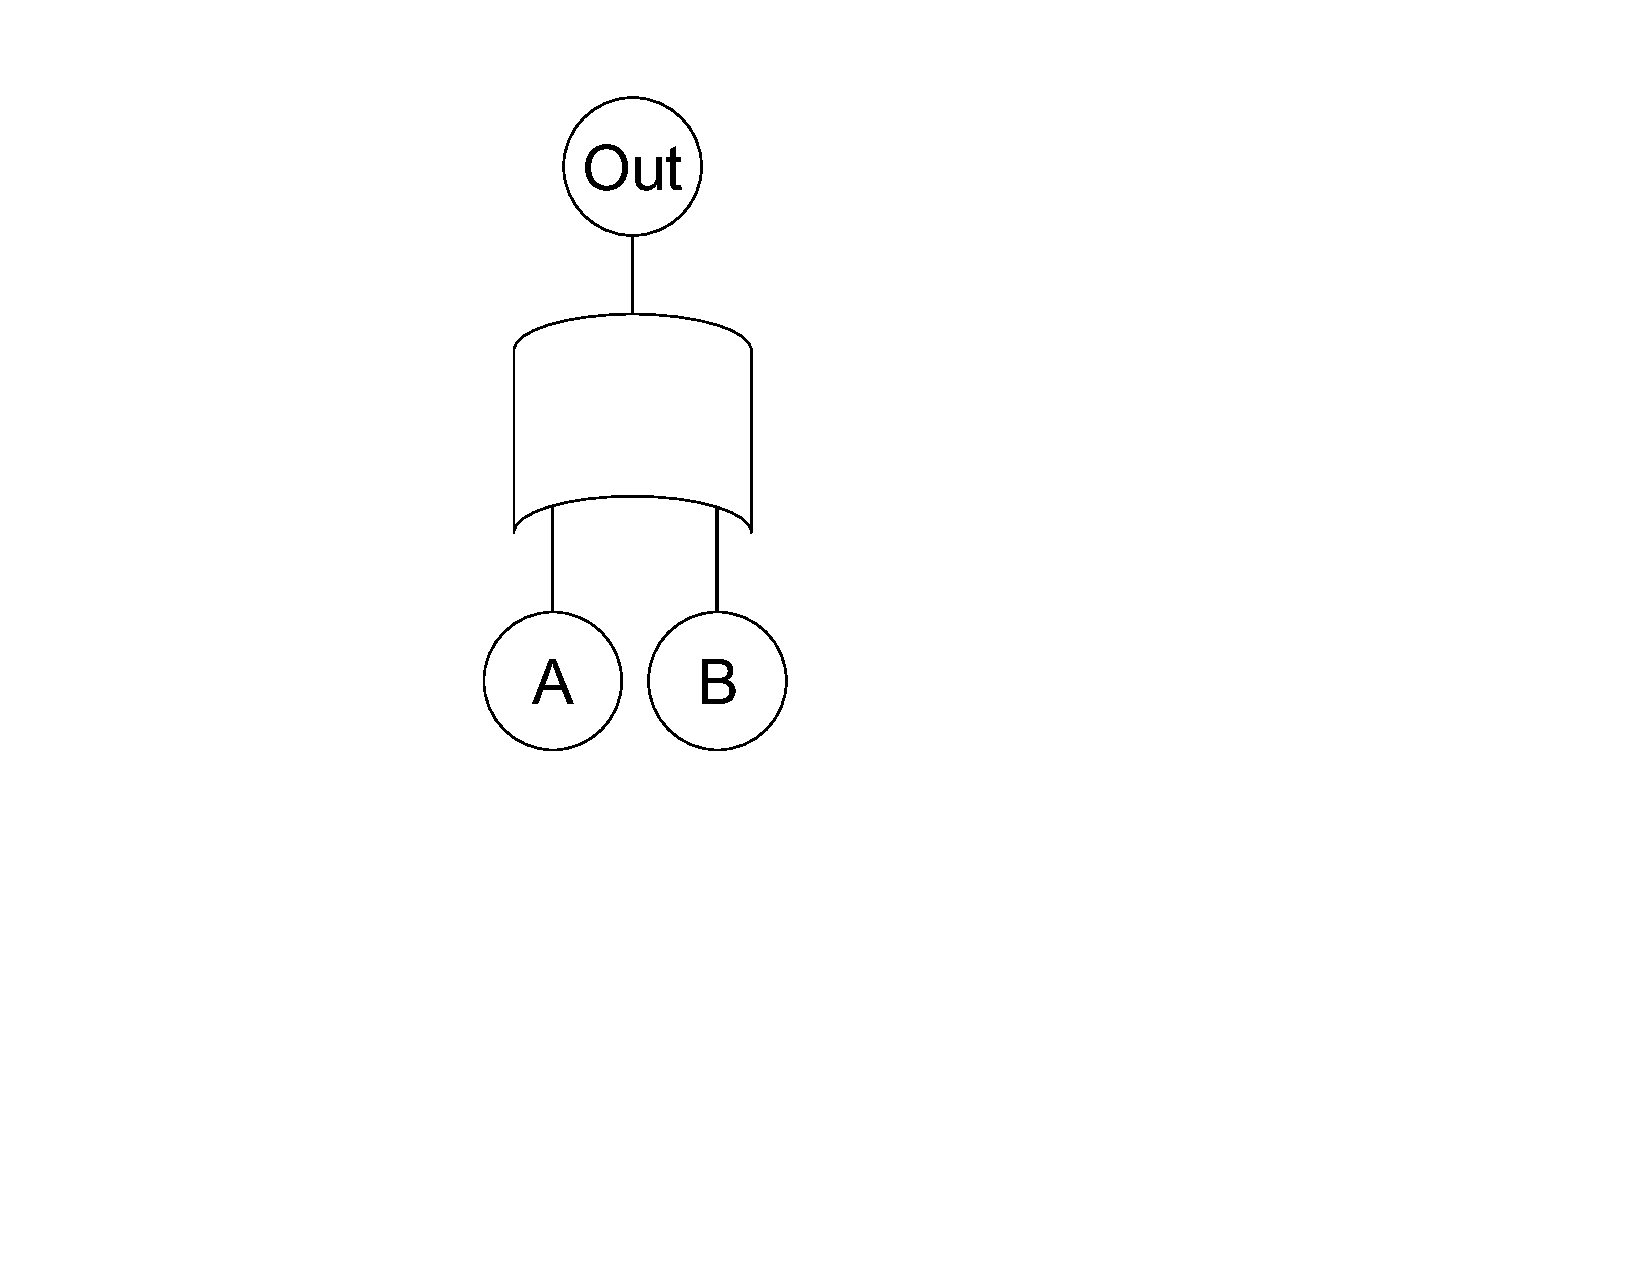
\includegraphics[scale=0.3]{andGate.pdf}
    \label{fig:sub2}
  \end{subfigure}
  \caption{Components A and B in a series configuration (left) and associated Fault-Tree (right).}
  \label{fig:chebyshev}
\end{figure}

\begin{figure}
    \centering
    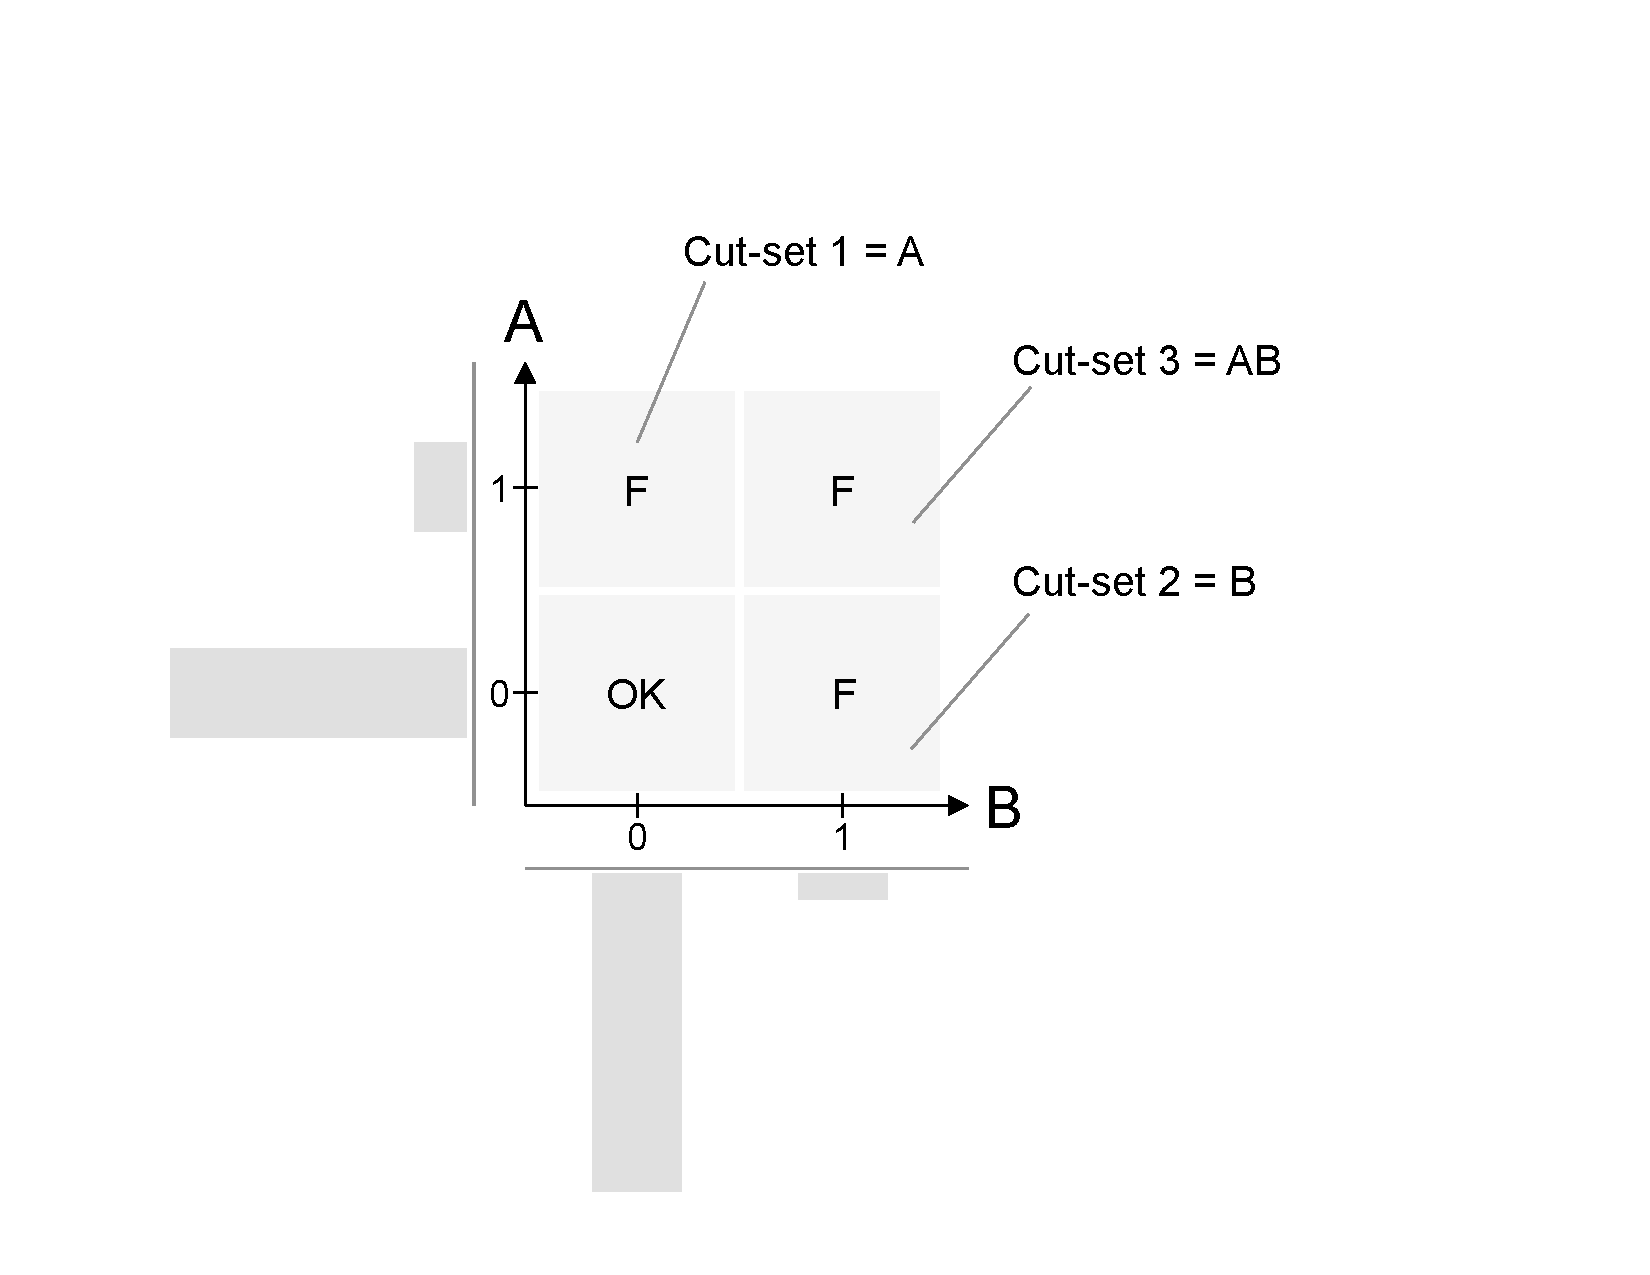
\includegraphics[scale=0.4]{2D.pdf}
    \caption{}
    \label{fig:2Danalogy}
\end{figure} 




\section{Data Mining}
\label{sec:dataMining}

Data mining is a fairly generic concept that entails the generation of information/knowledge 
from data sets.  The process of generation of information/knowledge can be performed in various 
ways depending on the type of application but it possible to classify all data analysis approaches 
into four categories:
\begin{itemize}
  \item ROM: ROM algorithms aim to reduce to the complexity of the data by 
        finding a mathematical objects that emulate the behavior of the data by learning its input/output 
        relations and reconstructing such relations through a regression/interpolation based approach
  \item Dimensionality reduction: this category includes all methods than aim to reduce the dimensionality 
        of the data set and project the original data into a reduced space
  \item Clustering: algorithms in this category partition the data based on a set of defined similarity measures
  \item Data searching: identify the closest data point in a database given a reference point. Once that 
        point has been found it is possible to infer properties of the reference point
\end{itemize} 

The range of applications that are of interest from an engineering point of view (and, hence, not 
limited to a typical RISMC application) are the following:
\begin{itemize}
  \item Analysis of data input-output relationship: this is the most relevant application within the RISMC 
        project, i.e., the identification of the connection between input parameters (which are stochastically 
        sampled) and the full temporal profile of the simulation. Using the system of equation (??), we want 
        to create a correlation between s and θ(t). While it is trivial to make a connection
        between input sampled parameters and static output parameters, such as max clad temperature or 
        average fluid speed, it gets tougher when we want to consider the full temporal profile of the 
        simulation
  \item Outlier identification: due to numerical limitations of system simulator codes (e.g., range of 
        validity for correlations), the outcome of a subset of simulation runs may contain wrong results. 
        When these limitations are reached, the temporal profile may contain anomalous behaviors. The
        objective of data mining would be to identify these anomalous behaviors, i.e. outliers. This would 
        dramatically increase the quality of the data being generated/analyzed
  \item Diagnosis/prognosis: while this application is not referenced in detail in this work, it is worth 
        highlighting that all data mining methods presented in this work can be used in an operating environment 
        to assist reactor operators to assess plant conditions and possible plant evolutions
        during an accident scenario. The basic idea would be use a large set of simulations generated for different 
        accident conditions as a database with the objective to constantly match the actual plant status. 
        Once a match has been established (i.e., a set of simulated scenarios match closely enough the actual and 
        past plant status) the operators can now:
        \begin{itemize}
          \item identify the possible causes that is generating the abnormal behavior in the plant (diagnosis)
          \item predict possible future evolutions of the accident scenarios (prognosis)
        \end{itemize} 
\end{itemize} 

In order to maintain the same standard throughout the paper, we introduce here the set of mathematical symbols 
and terminology. The types of data that are considered in this report are exclusively numerical data, i.e., 
data which consists of numbers of any format (either integer or double)
\footnote{This paper does not consider symbolic data sets, i.e., data which consists of symbols (e.g., text data)}. 
Given this,
we can represent a generic data set $\Xi$ as a collection of $N$ objects:
\begin{equation}
  \Xi = \{ H_1,\ldots,H_N \}  
  \label{eq:collection}
\end{equation}
Each object $H_n$ $(n=1,\ldots,N)$ lies in a multi-dimensional space $\Pi$: $H_n \in \Pi$ and $\Xi \subset \Pi$. 
From now on we will consider $\Pi$ 
as a metric space~\cite{}: $\Pi$ is a space where it is possible to define an arbitrary distance function, i.e., a 
metric.
Since we are dealing with numerical data in a multi-dimensional space we can say that $\Xi \subset \mathbb{R}$ 
where $D$ is the dimensionality of the space:
\begin{equation}
  H_n=[H_n^1,\ldots,H_n^d,\ldots,H_n^D ]
  \label{eq:collection_upd}
\end{equation}
We indicate with $x^d  (d=1,\ldots,D)$ each coordinate $d$ of $\Xi \subset \mathbb{R}$. 
Thus, each element $H_n^d$ of $H_n$ is the 
$d$ coordinate, i.e. dimension $x^d (d=1,\ldots,D)$, of the data point $H_n$.

\begin{figure}
  \centering
  \begin{subfigure}{.5\textwidth}
    \centering
    \includegraphics[scale=0.3]{hier_1.png}
    \label{fig:sub1}
  \end{subfigure}%
  \begin{subfigure}{.5\textwidth}
    \centering
    \includegraphics[scale=0.3]{hier_3.png}
    \label{fig:ABsystem}
  \end{subfigure}
  \caption{Components A and B in a series configuration (left) and its associated Fault-Tree (right).}
  \label{fig:ABsystem}
\end{figure}

\section{Clustering Algorithms}
\label{sec:clusteringAlgorithms}

From a mathematical viewpoint, clustering~\cite{SurveyClustering} aims is to find a partition
\begin{math} \mathbf{C}=\{C_{1},\ldots,C_{l},\ldots,{C_{L}}\}\end{math}
of $\Xi$ where each $C_{l}$ $(l=1,\ldots,L)$ is called a cluster. The partition
    $ \mathbf{C} $ of $ \mathbf{X} $
is such that:
    \begin{equation}\label{eq: ClassRequier}
        \begin{cases} \mathbf{C}_{l}\neq\varnothing, l=1,\ldots,L \\
                        \\
                     \bigcup_{l=1}^{L}\mathbf{C}_{l}= \Xi \\
        \end{cases}
    \end{equation}

Even though the number of clustering algorithms available in the literature is large, usually the most 
used ones when applied to time series are the following: Hierarchical~\cite{}, 
K-Means~\cite{} and Mean-shift~\cite{}.
Hierarchical algorithms build a hierarchical tree from the individual points (leaves) by progressively 
merging them into clusters until all points are inside a single cluster (root). 
Clustering algorithms such as K-Means and Mean-Shift, on the other hand, seek a single partition of 
the data sets instead of a nested sequence of partitions obtained by hierarchical methodologies. 

\subsection{Hierarchical}
\label{sec:hierarchical}

The hierarchical clustering is, along with the K-Means one (see Section~\ref{sec:kmeans}), the most basic 
clustering algorithms available in literature. Hierarchical algorithms organize data into a 
structure according to a proximity matrix in which each element $(j,k)$ is some measure of the 
similarity (or distance) between the items to which row $j$ and column $k$ correspond. 
Usually, the final result of these algorithms is a binary tree, also called dendrogram, 
in which the root of the tree represents the whole data set and each leaf is a data point. 
To show how hierarchical clustering works we will employ the data set pictured in 
Figure~\ref{}, i.e., a data set containing about one hundred points in a 2-dimensional space. 

Given a set of $N$ items to be clustered, and a $N \times N$ distance (or dissimilarity) matrix $\Delta$, 
the basic steps 
behind hierarchical clustering are the following:
\begin{enumerate}
  \item Assign each data point to a cluster, i.e., from $N$ data points, $N$ clusters are initialized, 
        each cluster contains just one data point. The distances among each cluster is the same as the
        distances between the data points they contain
  \item Determine the closest pair of clusters and merge them into a single cluster
  \item Determine the distances between the new cluster (obtained in Step 2) and the remaining clusters
  \item Repeat steps 2 and 3 until all items are clustered into a single cluster of size $N$
\end{enumerate}

\begin{figure}
    \centering
    \includegraphics[scale=0.2]{hier_2.png}
    \caption{}
    \label{fig:2Danalogy}
\end{figure}
  
\subsection{K-Means}
\label{sec:kMeans}  
  
The K-Means algorithm~\cite{} is probably the most simple clustering algorithm. The basic idea is to 
determine $K$ centers ($K$ is provided as an input variable) $\chi_k (k=1,\ldots,K)$: one center for each cluster.
At the beginning these centers are placed randomly in the feature space. The  next  step is to take 
each point of the data set and associate it to the nearest center $\chi_k$. At this point the centers $\chi_k$ 
are re-calculated as average of the data points associated to $\chi_k$. This data points and centers average 
step is repeated. As a result of this loop, the K centers change their location step by step until no 
more changes are done or, in other words, centers do not move any more. 

\subsection{Mean-Shift}
\label{sec:meanShift}

Mode-seeking approaches~\cite{} look at the density distribution of data points lying in a metric space. 
Clusters are viewed as regions of the space with high point density separated by regions of low
point density. Clusters can be identified by searching for regions of high density, called modes. 
For the comparison a Mode-seeking algorithm referred to as the Mean-Shift.

The Mean-Shift algorithm~\cite{} is a non-parametric iterative procedure that can be used to assign each 
point to one cluster center through a set of local averaging operations. The local averaging operations 
provide empirical cluster centers within the locality and define the vector which denotes the direction 
of increase for the underlying unknown density function.

The main idea is to consider each data point ??? of the dataset as an empirical 
distribution density function, or kernel, $K(\vec{x})$ distributed in a multidimensional space where 
regions with high data density (i.e., modes) correspond to local maxima of the multivariate kernel 
density estimate $f_{I}(\vec{x})$ \cite{CacoullosEstimation} (see Fig.~\ref{fig:densityfunc}).



\section{Time Dependent Data Mining}
\label{sec:timeDepDataMining}

At this point we can make step further: making 
the algorithms shown in Section~\ref{} useful to deal with time dependent data. 

Using same analogy presented for static data we aim to group scenario with similar 
temporal patterns.
An example is shown in Fig.~\ref{fig:TD-clustering} applied to a data set containing the time evolution 
of 1000 time series has been generated by randomly changing (through a Monte-Carlo 
sampling) three variables (i.e., $x,y,z$). 
We introduced a discontinuity in the temporal evolution of the time series 
depending if $x>=4$ or $x<4$.

\begin{figure}
    \centering
    \centerline{\includegraphics[scale=0.6]{TD-clustering.pdf}}
    \caption{Plot of a 1000 time series data set (right) and plot of the clustered data set colored 
             by the label assigned to each cluster.}
    \label{fig:TD-clustering}
\end{figure}

\begin{figure}
    \centering
    \centerline{\includegraphics[scale=0.4]{hist2Clusters.pdf}}
    \caption{Histograms of the sampled values for $Cluster_0$ and $Cluster_1$ (shown in Figure 4) that 
             created them and were captured by the clustering algorithm.}
    \label{fig:hist2Clusters}
\end{figure}

By using A clustering algorithm we want to partition the 1000 generated scenario into 
2 clusters (see Fig.~\ref{}). Note how the scenarios in each cluster have a very similar 
temporal behavior. Then, by looking at the histograms of the sampled variables $x,y,z$ 
for the scenarios contained in each cluster we were able to verify that $x$ was creating 
the splitting of the data set. 

Figure~\ref{} shows the histograms of $x$ for both clusters: 
for Cluster\_0 $x<4$ while $x>4$ for Cluster\_1. Note that we would not have been able to capture 
this discontinuity by considering only the end or max values of the time series.

Again, we will indicate with $\Lambda$ the data set generate by any of the methods mentioned above 
which contain $N$ time series~\footnote{In this paper we will indicate time series as simulation 
runs or histories} 
$TS_n (n=1,\ldots,N)$:
\begin{equation}
  \Lambda = \{ TS_1,\ldots,TS_N \}  
  \label{eq:collectionTS}
\end{equation}
To preserve generality, given the complexity of the data generated by simulation based PRA 
methods such as RISMC, we now assume that each scenario $Η_n$ contains three components: 
\begin{equation}
  TS_n = \{ \bm{\Theta}_n,\bm{\Sigma}_n,\bm{\Gamma}_n \}  
  \label{eq:collectionTS}
\end{equation}

These components are the following:
\begin{itemize}
  \item Continuous data $\bm{\Theta}_n$: this data contains the temporal evolution of each scenario, i.e., 
        the time evolution
        of the $M$ state variables $x_m^n (m=1,\ldots,M)$ (e.g., pressure and temperature at a specific 
        computational node). 
        All of these state variables change in time $t$ (where $t$~\footnote{This allows us to 
        maintain generality by having time series with different time lengths} ranges from 0 to $t_n$): 
        \begin{equation}
          \bm{\Theta}_n = {x_1^n,\ldots,x_M^n}  
          \label{eq:bigTheta}
        \end{equation}  
        where each $x_m^n$ is a an array of values having length $T_n$. Hence, $\bm{\Theta}_n$ can be viewed 
        as a $M \times T_n$ matrix .
  \item Discrete $\bm{\Sigma}_n$: which contains timing of events. Note that a generic event $E_i^n$ can occur:
        \begin{itemize}
          \item At a time instant $\tau_i$: in this case the event can be defined as $(E_i^n,\tau_i)$, or,
          \item Over a time interval $[\tau_i^\alpha,\tau_i^\omega]$: in this case the event can be defined 
                as $(E_i^n,[\tau_i^\alpha,\tau_i^\omega])$
        \end{itemize} 
  \item Set $\bm{\Gamma}_n$ of $V$ boundary conditions $BC_v^n (v=1,\ldots,V)$ and $U$ initial 
        conditions $BC_u^n (u=1,\ldots,U)$.
\end{itemize}


\subsection{Approaches}
\label{sec:timeDepDataMiningApproaches} 
Two possible paths  that can be followed to analyze time dependent data:
\begin{itemize}
  \item Path 1 (see Fig.~\ref{fig:approach1}): Employ classical clustering algorithms by transforming each time series as 
                                  a single multi-dimensional vector. Recall that algorithms such as K-Means 
                                  and Mean-Shift can naturally deal with multi-dimensional vectors, i.e., each data 
                                  point can be represented as a multi-dimensional vector. Following this, in this path
                                  each time series is converted into a multi-dimensional vector (as part of a 
                                  pre-processing step). This can be done, for example, through a polynomial or Fourier 
                                  transformation (see Section~\ref{}).
  \item Path 2 (see Fig.~\ref{fig:approach2}): Maintain the original format of the time series end employ clustering algorithms that 
                                  can receive in input a distance matrix (thus appropriate distance metrics needs to be 
                                  defined). Few algorithms, such the hierarchical and the DBSCAN clustering
                                  algorithms can received in input the solely distance matrix $\Delta=[\delta_{ij}]$ where each 
                                  element $\delta_{ij}$ represent the distance between time series $i$ and $j$.
\end{itemize}

The advantage of the first path is that it employs a large variety of clustering algorithms that can handle very complex 
data sets (i.e., data points clustered in complex shapes other than ellipsoidal). On the other side, the 
conversion of the time series prior the clustering may cause erroneous results if clustering
parameters are not chosen properly (e.g., if the time series are very similar to each other and a coarse 
representation is chosen).

The second path, however, since it employs algorithms which can accent as input the distance matrix $\Delta$, they do not 
require any data transformation. When dealing with time series data the most important parameter to be considered 
here is the distance metric chosen to determine each element $\delta_{ij}$ of $\Delta$.

\begin{figure}
    \centering
    \centerline{\includegraphics[scale=0.4]{approach1.pdf}}
    \caption{Analysis of time-dependent data using static representation conversion.}
    \label{fig:approach1}
\end{figure}

\begin{figure}
    \centering
    \centerline{\includegraphics[scale=0.4]{approach2.pdf}}
    \caption{Analysis of time-dependent data using distance matrix based algorithms (e.g., Hierarchical).}
    \label{fig:approach2}
\end{figure}


\section{Data Pre-processing}
\label{sec:preProcessing} 

\subsection{Data Normalization}
\label{sec:dataNormalization} 

Depending on the application, the data set may need to be pre-processed. A common pre-processing method is the 
Z-normalization procedure: each variable $x_m^n$ of $\bm{\Theta}_n$ is transformed into $\tilde{x}_m^n$:

\begin{equation}
  \tilde{x}_m^n = \dfrac{(x_m^n-mean[x_m^n])}{stdDev[x_m^n]}  
  \label{eq:Znormalization}
\end{equation}

where $mean[x_m^n]$ and $stdDev[x_m^n]$ represent the mean and the standard deviation of $x_m^n$. 
This transformation provides an equal importance to every $x_m^n$ and it compensates for amplitude offset 
and scaling effects when distance between time series is computed.

\subsection{Data Smoothing}
\label{sec:dataSmoothing} 

In case the time-series are affected by noise, it might be worthwhile to smooth the time series using classical 
filtering and regression techniques so that the noise is filtered out and the series information is maintained. 
A commonly used de-noising or filtering technique is the kernel-regression technique.
This simple technique starts from the raw data $\bm{\Theta}_n$ which is time dependent (i.e., $\bm{\Theta}_n(t)$) 
and it generates the regressed term $\bm{\tilde{\Theta}}_n$ as follows:

\begin{equation}
  \bm{\tilde{\Theta}}_n = \dfrac{\sum_{t=0}^{T_n} K(t-t') \bm{\Theta}_n}{\sum_{t=0}^{T_n} K(t-t')} 
  \label{eq:smoothing}
\end{equation}
[review this!!!]
where $K(t-t')$ is the kernel used to smooth $\bm{\Theta}_n$.

\begin{figure}
    \centering
    \centerline{\includegraphics[scale=0.4]{figure_filtered.png}}
    \caption{pppp}
    \label{fig:smoothing}
\end{figure}

\subsection{Data Resampling}
\label{sec:dataResampling} 

Another operation that can be performed in the pre-processing is the re-sampling of $\bm{\Theta}_n$. Recall that 
$\bm{\Theta}_n$ contains the values of the time dependent data variables ${x_1^n,\ldots,x_M^n}$ sampled at specific 
time instants. 
The re-sampling operation aims to reduce those time instants by choosing a new set of time instants (typically a 
smaller set) that preserves the information content of the $\bm{\Theta}_n$.
The motivations behind the choice of this step are the following: less memory intensive and faster computations.
Several re-sampling strategies can be employed:
\begin{itemize}
  \item Uniform: $N$ sample points ($N$ is provided as input) are uniformly located along the time axis
  \item First derivative: $N$ sample points ($N$ is provided as input) concentrated in regions with higher values 
        of the first derivative
  \item Second derivative: $N$ sample points ($N$ is provided as input) concentrated in regions with higher values 
        of the second derivative
  \item samples with derivative greater than fixed value
\end{itemize}
  
\section{Data Representation}
\label{sec:dataRepresentation}   
  
One of the most fundamental modeling choices regarding time dependent data is how each time series is actually 
represented in the data mining process. Reference~\cite{} provides a broad analysis of the
many representation methods. Some of these methods have been implemented in RAVEN; the choice of these implemented methods 
was based on their effectiveness on nuclear engineering applications. In the following sub-sections we will present 
these methods in mode detail along with some preliminary results obtained by RAVEN. 

\subsubsection{Real-valued}
\label{sec:realValued}

The original format of the time series is maintained. This approach does not require any prior knowledge from 
the user so it can be considered a fail-safe approach. On the other side this method
(depending on the data set) can be memory and computationally intensive.

\subsubsection{Polynomial}
\label{sec:polynomial}

The time series is approximated by a Taylor polynomial function (see~\cite{}) up to a 
fixed degree and the vector of coefficients are retained as representatives for the time series. 
Recall that $\bm{\Theta}_n = {x_1^n,\ldots,x_M^n}$ contains the temporal evolution of a set of $M$ 
variables (i.e., $x_1^n = x_1^n (t)$), 
for the Taylor case for example, the approximation is performed as follows for each $x_1^n(t)$:
\begin{equation}
  x_1^n(t) \approx \sum_{\varsigma=0}^C c_\varsigma t^\varsigma
  \label{eq:polynomial}
\end{equation}
The representation process using Taylor expansion replace $x_1^n(t)$ with a vector having dimensionality $C+1$ 
containing the coefficients $c_\varsigma (\varsigma=0,\ldots,C)$.

\subsubsection{Chebyshev}
\label{sec:Chebyshev}

The Chebyshev representation follows exact principle presented above for the Taylor case (see~\cite{}):
\begin{equation}
  x_1^n(t) \approx (\sum_{\varsigma=0}^{C-1} c_\varsigma T_\varsigma) - \frac{1}{2} c_0
  \label{eq:chebyshev}
\end{equation}
where $T_\varsigma(t)$ is the Chebyshev polynomial of order $\varsigma$:
\begin{equation}
\begin{array}{r@{}l}
  T_0(t)&{}=1 \\
  T_1(t)&{}=t \\
  T_2(t)&{}=2 t^2-1) \\
  T_3(t)&{}=4 t^3-3t \\
  T_4(t)&{}=8 t^4-8 t^2+1) \\
        &{}\ldots \\
  T_{\varsigma+1}(t)&{}=2 t T_\varsigma(t)-T_{\varsigma-1}(t)
  \label{eq:ChebyshevPolynomialCoeffs}
\end{array}
\end{equation}
The representation process using Chebyshev expansion replace $x_1^n(t)$ with a vector having dimensionality $C+1$ 
containing all coefficients $c_\varsigma (\varsigma=0,\ldots,C)$. 

\begin{figure}
  \centering
  \begin{subfigure}{.5\textwidth}
    \centering
    \includegraphics[scale=0.3]{cheb1.png}
    \label{fig:sub1}
  \end{subfigure}%
  \begin{subfigure}{.5\textwidth}
    \centering
    \includegraphics[scale=0.3]{cheb1.png}
    \label{fig:sub2}
  \end{subfigure}
  \caption{Chebyshev approximation of a time series for several polynomial degrees.}
  \label{fig:chebyshev}
\end{figure}

\subsubsection{Legendre}
\label{sec:Legendre}

The Legendre polynomials are polynomials (see~\cite{}) of the following form:
\begin{equation}
\begin{array}{r@{}l}
  P_0(t)&{}=1 \\
  P_1(t)&{}=t \\
  P_2(t)&{}=\frac{2 t^2-1)}{2} \\
  P_3(t)&{}=\frac{5 t^3-3t}{2} \\
  P_4(t)&{}=\frac{35 t^4-30 t^2+3}{8} \\
        &{}\ldots \\
  P_{\varsigma+1}(t)&{}=\frac{(2 \varsigma-1)  t P_(\varsigma-1)(t)-(\varsigma-1) P_(\varsigma-2) (t)}{\varsigma}
  \label{eq:LegendrePolynomialCoeffs}
\end{array}
\end{equation}

The representation process using Legendre expansion replace $x_1^n (t)$ with a vector having dimensionality $C+1$ 
containing all coefficients $c_\varsigma  (\varsigma=0,…,C)$. 

\subsubsection{Laguerre}
\label{sec:Laguerre}
The Laguerre polynomials $L_n(t)$ are polynomials (see~\cite{}) of the following form::
\begin{equation}
\begin{array}{r@{}l}
  L_0(t)&{}=1 \\
  L_1(t)&{}=1-t \\
        &{}\ldots \\
  (n+1) L_n(t)&{}-(2n+1-t) L_n(t)+n L_{n-1}(t)=0
  \label{eq:LaguerrePolynomialCoeffs}
\end{array}
\end{equation}

\subsubsection{Hermite}
\label{sec:Hermite}

The Hermite polynomials $H_n(t)$ are polynomials of the following form (see~\cite{}):
\begin{equation}
\begin{array}{r@{}l}
  H_0(t)&{}=1 \\
  H_1(t)&{}=t \\
        &{}\ldots \\
  H_{n+1}(t)&{}-2 t H_n(t)+2 n H_{n-1}(t)=0
  \label{eq:HermitePolynomialCoeffs}
\end{array}
\end{equation}

\subsubsection{Discrete Fourier Transform}
\label{sec:fourier}

Similar to the polynomial representation, the time series is approximated by a Fourier series and the series coefficients 
are retained as representatives for the time series. The Fourier series is as follows 
\begin{equation}
  x_1^n(t) \approx \frac{a_0}{2} (\sum_{\varsigma=1}^{C} (a_\varsigma cos(\varsigma t) + b_\varsigma sin(\varsigma t)) 
  \label{eq:fourier}
\end{equation}

\begin{figure}
  \begin{subfigure}{.5\linewidth}
    \centering
    \includegraphics[scale=0.3]{fourier1.png}
  \end{subfigure}%
  \begin{subfigure}{.5\linewidth}
    \centering
    \includegraphics[scale=0.3]{fourier2.png}
  \end{subfigure}
  \caption{Fourier approximation of a time series for several polynomial degrees.}
  \label{fig:fourier}
\end{figure}

\subsubsection{Singular Value Decomposition (SVD)}
\label{sec:svd}

This method performs an eigenvalues and eigenvectors decomposition of $\bm{\Theta}_n$ and selects a reduced set of eigenvectors. 
Each time series $Η_n$ is represented by the coefficients associated to each eigenvector. 
Note that this decomposition must be performed on all time-series as a whole since SVD decomposition is performed 
on the covariance matrix which is calculated by considering all set of time series and not one time series separately. 

This is performed for each $x_m (m=1,\ldots,M)$ independently by:
\begin{enumerate}
  \item Normalizing the data: zero mean and unit variance (see Section~\ref{})
  \item Resampling the data set so that all time series have been sampled on the exact same time instants
  \item Determining the covariance matrix
  \item Performing SVD of the covariance matrix, i.e., eigenvalues and eigenvectors decomposition~\cite{}. 
        Note that each eigenvector is a time series sampled at the same time instants of the original time series. 
        The eigenvectors can be ranked based on the associated eigenvalues: the space
        reduction can be performed by considering the eigenvector with higher eigenvalues 
  \item Projecting the original time series into the eigenvectors space (either reduced or not) and using the projection 
        coefficients as time series representation format.
\end{enumerate}
 
\begin{figure}
  \begin{subfigure}{.5\linewidth}
    \centering
    \includegraphics[scale=0.3]{SVD1.png}
  \end{subfigure}%
  \begin{subfigure}{.5\linewidth}
    \centering
    \includegraphics[scale=0.3]{SVD3.png}
  \end{subfigure}
  \caption{[]}
  \label{fig:svd}
\end{figure}  

\begin{figure}
    \centering
    \centerline{\includegraphics[scale=0.4]{SVD4.png}} 
    \caption{[]}
    \label{fig:SVDcumulative}
\end{figure} 
  

\section{Measuring similarities}
\label{sec:similarities}

An important modeling choice when dealing with time series is the type of similarity 
metric employed to measure similarity among time series: a distance metric. 
Similarly to any distance metric defined in an euclidean space, 
a distance metric $d(S,Q)$ between two time series $S$ and $Q$ must obey the following rules:
\begin{equation}
  \begin{cases}
    d(S,S) = 0 \\
    d(S,Q) = d(Q,S) \\ 
    d(S,Q) = 0  \Longleftrightarrow  S=Q \\ 
    d(S,Q) \leq d(S,K) + d(K,Q) 
  \end{cases}
  \label{eq:distanceRules}
\end{equation}

When dealing with time series, the two metrics are the most commonly used: Euclidean and 
Dynamic Time Warping (DTW) distance. These distances are described in the next two subsections for
the univariate case, i.e., two time series Q and S where their continuous part has $M=1$. 
The more generic case, i.e., multivariate case, can be easily expanded from what is shown below.

\subsection{Euclidean Distance}
\label{sec:euclidean}

Given two univariate time series S and Q having identical length (i.e., $T_S=T_Q$) the Euclidean 
distance $d_2(S,Q)$ is defined as:
\begin{equation}
  d_2(S,Q) = \sqrt{ \sum_{t=0}^{T_s} (x_1^S(t)-x_1^Q(t))}
  \label{eq:euclidean}
\end{equation}

\begin{figure}
    \centering
    \includegraphics[scale=0.3]{L2.pdf}
    \caption{}
    \label{fig:2Danalogy}
\end{figure} 

Note that this distance metric requires identical 

\subsection{DTW Distance}
\label{sec:dtw}


This distance can be viewed as a natural extension of the Euclidean distance applied to time series~\cite{}. 
Given two univariate time series $S$ and $Q$ having length $T_S$ and $T_Q$ respectively, the distance value 
$d_DTW (S,Q)$ is calculated by following these two steps:
\begin{enumerate}
  \item Create a matrix $D=[d(i,j)]$ having dimensionality $T_S \times T_Q$ where each element of $D$ (see Fig.~\ref{} for 
        the time series shown in Fig.~\ref{}) is calculated as $d(i,j)=(x_1^S[i]-x_1^Q[j])^2$ for
        $i=1,\ldots,T_S$ and $j=1,\ldots,T_Q$.
  \item Search a continuous path $w_k|_1^K$ in the matrix $D$ that, starting from $(i,j)=(0,0)$, it ends at 
        $(i,j)=(T_S,T_Q)$ and it minimizes the sum of all the $K$ elements $w_k=(d(i,j))_k$ of this
       path (see blue line in Fig.~\ref{}):
      \begin{equation}
        d_DTW(S,Q) = min⁡(\sum_{k=1}^{K} w_k)
        \label{eq:dtw}
      \end{equation}       
       Each element of the path corresponds to a specific black segment in Fig.~\ref{}. This metric can capture 
       similarities between time series that are shifted in time.
\end{enumerate}

\begin{figure}
  \centering
  \begin{subfigure}{.5\textwidth}
    \centering
    \includegraphics[scale=0.25]{DTW_path.pdf}
  \end{subfigure}%
  \begin{subfigure}{.5\textwidth}
    \centering
    \includegraphics[scale=0.25]{DTW.pdf}
  \end{subfigure}
  \caption{.}
  \label{fig:DTW}
\end{figure}


\section{Test Cases}
\label{sec:testCases}

\subsection{Pump Controller}
\label{sec:pumpController}

The first test case considers a pump controller model for a hypothetical simplified PWR model 
(see Figure 15) which consists of the following components: Reactor core (RX), Motor operated 
pump, Pump digital controller, Heat exchanger (HX).
This system is responsible to remove the decay heat generated from the core (RX) in order to 
avoid damage of the core itself. The objective is to maintain the temperature in the reactor 
core between 1500 C and 1600 C. The top-events are thus the following:
\begin{itemize}
  \item Success: final temperature between 1500 C and 1600 C
  \item Failure-high: final temperature greater than 3000 C
  \item Failure-low: final temperature lower than 1600 C
\end{itemize}

While we assumed that both the HS and the pump are perfectly reliable components (i.e., no 
failure can be introduced), using~\cite{} as a references, the digital pump controller 
reliability model has been performed using a continuous time Markov Chain formulation.

In more detail, the controller has been modeled using 4 states (see. Fig.~\ref{}):
\begin{itemize}
  \item State 0 - Operating: controller operating as designed
  \item State 1 - Failed closed: controller failed by sending close signal to pump (i.e., pump not running)
  \item State 2 - Failed stuck: controller failed by sending oldest valid signal to pump
  \item State 3 - Failed random: controller failed by sending close signal to pump
\end{itemize}
For the scope of this report we have assumed a constant (in time) failure rate $\lambda$ 
for all three transitions 
shown in Fig.~\ref{}. The scope of this exercise is to identify the impact of both
timing and type of failure on the system dynamics.

\begin{figure}
  \begin{subfigure}{.5\linewidth}
    \centering
    \includegraphics[scale=0.7]{controller.pdf}
  \end{subfigure}%
  \begin{subfigure}{.5\linewidth}
    \centering
    \includegraphics[scale=0.7]{Markov.pdf}
  \end{subfigure}
  \caption{Pump controller test case: scheme of the system considered and continuous time Markov model for the pump controller.}
  \label{fig:pumpController}
\end{figure}

In order to perform such analysis the model has been coded as a RAVEN external model (i.e., Python based code) 
which determine the temporal profile of core temperature give the two stochastic parameters: Pump controller 
failure time and Pump controller failure mode
The dynamic of the system has been modeled using basic mass and energy conservation laws so no effective 
engineering conclusions can be gathered by this example. An example of scenario where no pump failure occurs 
is shown in Fig.~\ref{}. Note that the transient has been divided along the temporal axis in 5 regions where:
\begin{itemize}
  \item Pump is ON in regions 1, 3 and 5
  \item Pump is OFF in regions 2 and 4
\end{itemize}

\begin{figure}
    \centering
    \centerline{\includegraphics[scale=0.3]{scenarioController.pdf}} 
    \caption{Pump controller: example of scenario where no pump failure occurs.}
    \label{fig:scenarioController}
\end{figure}

By using RAVEN we sampled the two stochastic parameters (see the histograms of these variables in Fig.~\ref{}) 
using a Monte-Carlo algorithm and generated 1500 simulations as shown in Fig.~\ref{}.

\begin{figure}
    \centering
    \centerline{\includegraphics[scale=0.4]{controllerAllScen.pdf}} 
    \caption{Pump controller: plot of the 1500 histories generated by RAVEN.}
    \label{fig:controllerAllScen}
\end{figure}

By observing only static values such as max or final temperature (see Fig.~\ref{}) it is not really possible to 
extract valuable information from the data set. 
For the analysis of this dataset we have chosen to use hierarchical clustering using Euclidean distance as 
distance metrics. The dendrogram obtained is shown in Fig.~\ref{}. From this dendrogram it is
clearly possible to identify 3 clusters which lead us to choose a separation level equal to 10; 
the plot of the scenarios colored by the clustering label value is shown in Fig.~\ref{}.

\begin{figure}
    \centering
    \centerline{\includegraphics[scale=0.4]{controllerInitialHist.pdf}} 
    \caption{Histograms of max (left) and final (right) temperature of the simulations shown in Fig.~\ref{}}
    \label{fig:controllerInitialHist}
\end{figure}

\begin{figure}
    \centering
    \centerline{\includegraphics[scale=0.4]{controllerDend1.pdf}} 
    \caption{Dendogram obtained using hierarchical clustering (euclidean distance) for the dataset 
             shown in Fig.~\ref{}}
    \label{fig:controllerDend1}
\end{figure}

\begin{figure}
    \centering
    \centerline{\includegraphics[scale=0.4]{controllerClusteredScen.pdf}} 
    \caption{Plot of the 1500 histories generated by RAVEN (see Fig.~\ref{}) colored based on the labels assigned 
             by the hierarchical clustering (see Fig.~\ref{}).}
    \label{fig:controllerClusteredScen}
\end{figure}

\begin{figure}
  \centering
  \begin{minipage}{.33\textwidth}
  \centering
  \includegraphics[width=\linewidth]{1-Clustered_HS_1_line.png}
  \end{minipage}\hfill
  \begin{minipage}{.33\textwidth}
  \centering
  \includegraphics[width=\linewidth]{1-HistTime_1_histogram.png}
  \end{minipage}\hfill
  \begin{minipage}{.33\textwidth}
  \centering
  \includegraphics[width=\linewidth]{1-HistMode_1_histogram.png}
  \end{minipage}
  \caption{Cluster 1 (see Fig.~\ref{}): plot of the histories (left), histograms of failure mode (center) 
           and failure time (right).}
  \label{fig:pump_cluster1}
\end{figure}

\begin{figure}
  \centering
  \begin{minipage}{.33\textwidth}
  \centering
  \includegraphics[width=\linewidth]{1-Clustered_HS_2_line.png}
  \end{minipage}\hfill
  \begin{minipage}{.33\textwidth}
  \centering
  \includegraphics[width=\linewidth]{1-HistTime_2_histogram.png}
  \end{minipage}\hfill
  \begin{minipage}{.33\textwidth}
  \centering
  \includegraphics[width=\linewidth]{1-HistMode_2_histogram.png}
  \end{minipage}
  \caption{Cluster 2 (see Fig.~\ref{}): plot of the histories (left), histograms of failure mode (center) 
           and failure time (right).}
  \label{fig:pump_cluster2}
\end{figure}

\begin{figure}
  \centering
  \begin{minipage}{.33\textwidth}
  \centering
  \includegraphics[width=\linewidth]{1-Clustered_HS_3_line.png}
  \end{minipage}\hfill
  \begin{minipage}{.33\textwidth}
  \centering
  \includegraphics[width=\linewidth]{1-HistTime_3_histogram.png}
  \end{minipage}\hfill
  \begin{minipage}{.33\textwidth}
  \centering
  \includegraphics[width=\linewidth]{1-HistMode_3_histogram.png}
  \end{minipage}
  \caption{Cluster 3 (see Fig.~\ref{}): plot of the histories (left), histograms of failure mode 
           (center) and failure time (right).}
  \label{fig:pump_cluster3}
\end{figure}

\begin{figure}
    \centering
    \centerline{\includegraphics[scale=0.4]{1-Clustered_HS_sub_line.png}} 
    \caption{Plot of the histories belonging to Cluster 1 (see Fig.~\ref{}) colored based on the 
             labels assigned by the hierarchical clustering (see Figure 69).}
    \label{fig:controllerDend1}
\end{figure}

The analysis of the obtained clusters is summarized in Fig.~\ref{} (Cluster 1), Fig.~\ref{} (Cluster 2), 
Fig.~\ref{} (Cluster 3). In order to describe the obtained results we refer also to Fig.~\ref{}:
\begin{itemize}
  \item Cluster 1 (see Fig.~\ref{}) contains a large number of scenarios that lead to both ``failure-high'' and 
        ``success'' top-events and no other particular information can be deduced
  \item Cluster 2 (see Fig.~\ref{}) and 3 (see Fig.~\ref{}8) contain scenarios where pump controller in 
        State 2 (i.e., stuck) while the pump was actually ON in region 1 and 3 respectively (Fig.~\ref{}). They
        are all leading to the “failure-low” top-event Given the fact that cluster 1 contains too much variety 
        of scenarios, we performed hierarchical clustering on just the scenarios belonging to Cluster 1:
        i.e., sub-clustering. The obtained dendrogram is shown in Fig.~\ref{}. In this case, 5 clusters 
        were obtained; the plot of the scenarios colored by the clustering label value is shown in Fig.~\ref{}.
\item 
\end{itemize}

The analysis of the obtained clusters is summarized in Fig.~\ref{} (Cluster 1), Fig.~\ref{} (Cluster 2), 
Fig.~\ref{} (Cluster 3), Fig.~\ref{} (Cluster 4) and Fig.~\ref{} (Cluster 5):
\begin{itemize}
  \item Clusters 1, 2, 4 and 5 (see Fig.~\ref{}, Fig.~\ref{}, Fig.~\ref{} and Fig.~\ref{} respectively) 
        contain scenarios where pump controller failed in any of the three modes (closed, stuck and
        random) but did not lead to the failure-high top event 
  \item Cluster 3 (see Fig.~\ref{}) contains scenarios where pump controller failed in only two modes 
        (closed and random). Note that:
  \begin{itemize}
    \item Pump failed in the first time region
    \item Controller failure random did not lead failure-high top event; however, controller failure closed 
          lead to very high core temperatures (including 3000 C)
   \end{itemize}
   This cluster contains scenarios leading to failure-high and success top events. Note that if controller 
   failure occurs prior to about 115 min that the simulation leads to failure-high top event.
\end{itemize}

In summary, using the analytical model data set we were able to gather the following information:
\begin{itemize}
  \item Failure-high top event can be reached if controller failure to state 1 (i.e., failure closed) occurs 
        prior to 115 min 
  \item Failure-low top event can be reached if controller failure to state 2 (i.e., failure stuck) occurs 
        in the time regions 1 and 3
  \item Controller failure to state 3 (i.e., failure random) do not lead to any failure top event independently 
        of the controller failure time
  \item For these controller failure events the core temperatures are between 1500 C and 3000 C:
  \begin{itemize}
    \item Controller failure to state 1 (i.e., failure closed) after to 115 min
    \item Controller failure to state 2 (i.e., stuck) in time regions 2, 4 and 5
  \end{itemize}
\end{itemize}

\begin{figure}
  \centering
  \begin{minipage}{.33\textwidth}
  \centering
  \includegraphics[width=\linewidth]{1-Clustered_HS_sub_1_line.png}
  \end{minipage}\hfill
  \begin{minipage}{.33\textwidth}
  \centering
  \includegraphics[width=\linewidth]{1-HistTimeSub_1_histogram.png}
  \end{minipage}\hfill
  \begin{minipage}{.33\textwidth}
  \centering
  \includegraphics[width=\linewidth]{1-HistModeSub_1_histogram.png}
  \end{minipage}
  \caption{Cluster 1 (see Fig.~\ref{}): plot of the histories (left), histograms of failure mode 
           (center) and failure time (right).}
  \label{fig:pump_cluster_1_1}
\end{figure}

\begin{figure}
  \centering
  \begin{minipage}{.33\textwidth}
  \centering
  \includegraphics[width=\linewidth]{1-Clustered_HS_sub_2_line.png}
  \end{minipage}\hfill
  \begin{minipage}{.33\textwidth}
  \centering
  \includegraphics[width=\linewidth]{1-HistTimeSub_2_histogram.png}
  \end{minipage}\hfill
  \begin{minipage}{.33\textwidth}
  \centering
  \includegraphics[width=\linewidth]{1-HistModeSub_2_histogram.png}
  \end{minipage}
  \caption{Cluster 2 (see Fig.~\ref{}): plot of the histories (left), histograms of failure mode 
           (center) and failure time (right).}
  \label{fig:pump_cluster_1_2}
\end{figure}

\begin{figure}
  \centering
  \begin{minipage}{.33\textwidth}
  \centering
  \includegraphics[width=\linewidth]{1-Clustered_HS_sub_3_line.png}
  \end{minipage}\hfill
  \begin{minipage}{.33\textwidth}
  \centering
  \includegraphics[width=\linewidth]{1-HistTimeSub_3_histogram.png}
  \end{minipage}\hfill
  \begin{minipage}{.33\textwidth}
  \centering
  \includegraphics[width=\linewidth]{1-HistModeSub_3_histogram.png}
  \end{minipage}
  \caption{Cluster 3 (see Fig.~\ref{}): plot of the histories (left), histograms of failure mode 
           (center) and failure time (right).}
  \label{fig:pump_cluster_1_3}
\end{figure}

\begin{figure}
  \centering
  \begin{minipage}{.33\textwidth}
  \centering
  \includegraphics[width=\linewidth]{1-Clustered_HS_sub_4_line.png}
  \end{minipage}\hfill
  \begin{minipage}{.33\textwidth}
  \centering
  \includegraphics[width=\linewidth]{1-HistTimeSub_4_histogram.png}
  \end{minipage}\hfill
  \begin{minipage}{.33\textwidth}
  \centering
  \includegraphics[width=\linewidth]{1-HistModeSub_4_histogram.png}
  \end{minipage}
  \caption{Cluster 4 (see Fig.~\ref{}): plot of the histories (left), histograms of failure mode 
           (center) and failure time (right).}
  \label{fig:pump_cluster_1_4}
\end{figure}


\begin{figure}
  \centering
  \begin{minipage}{.33\textwidth}
  \centering
  \includegraphics[width=\linewidth]{1-Clustered_HS_sub_5_line.png}
  \end{minipage}\hfill
  \begin{minipage}{.33\textwidth}
  \centering
  \includegraphics[width=\linewidth]{1-HistTimeSub_5_histogram.png}
  \end{minipage}\hfill
  \begin{minipage}{.33\textwidth}
  \centering
  \includegraphics[width=\linewidth]{1-HistModeSub_5_histogram.png}
  \end{minipage}
  \caption{Cluster 5 (see Fig.~\ref{}): plot of the histories (left), histograms of failure mode 
           (center) and failure time (right).}
  \label{fig:pump_cluster_1_5}
\end{figure}


\section*{References}

\bibliography{main}

\end{document}